\chapter{The Built-in Theories of \lclam\ }
\label{theories}


\section{Introduction}
\lclam\ is best known as a inductive proof planner.  The object of
this chapter is to give an overview of the implementation of methods
for induction in \lclam.  It also discusses briefly some of the other
built-in theory files.

\section{The Proof Strategy for Induction and Rippling}
The proof strategy for induction can be seen in 
figure~\ref{fig:induction_strategy}.  
\begin{figure}[htb]
\begin{center}
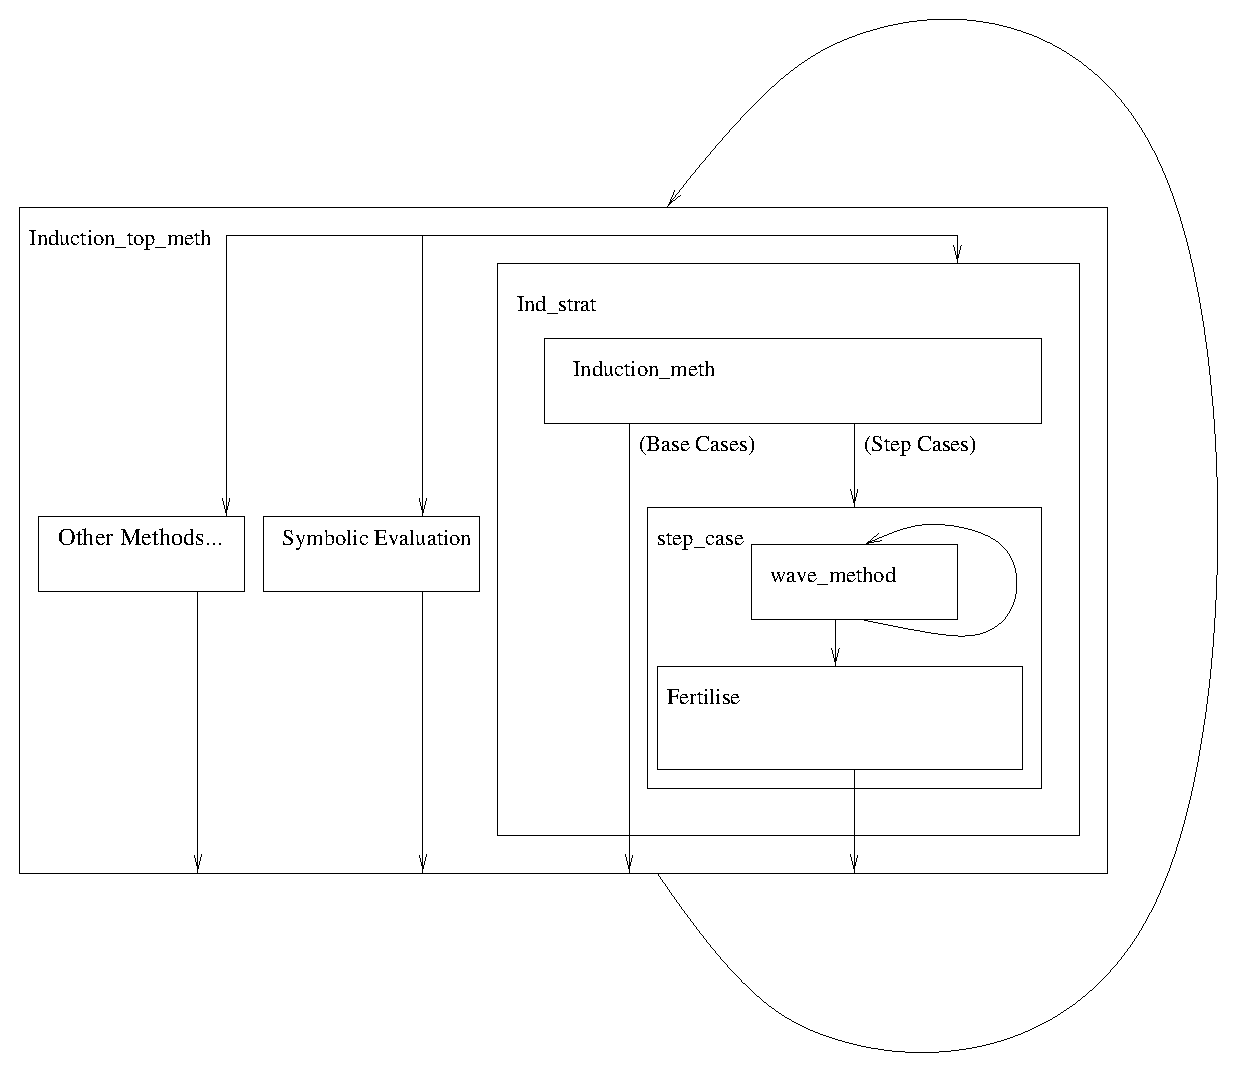
\epsfig{file=ind_strat.eps, width=4.8in}
\end{center}
\caption{The Proof Strategy for Induction}
\label{fig:induction_strategy}
\end{figure}
This is implemented as a selection of atomic and compound methods.
The diagram shows a top level repeat which attempts a disjunction of
methods.  These include basic tautology checking, generalisation of
common subterms and also symbolic
evaluation and the induction strategy ({\tt ind\_strat}).  Within the
induction strategy, the induction method
performs ripple
analysis~\cite{ind-chap-ref2} to choose an induction scheme (from a
selection specified in \lclam's theories) and produces subgoals for
base and step cases.  The base cases
are passed out to the repeat of the top level strategy.
The step cases are annotated with \emph{skeletons} and
\emph{embeddings} (described 
below) and then the wave method is repeatedly applied to them followed 
by fertilisation (exploitation of the induction hypothesis).
Annotations are then removed.  The methods ({\tt set\_up\_ripple} and
{\tt post\_ripple}) which place and remove annotations are omitted
from the diagram.  The results are then passed out to the top level
strategy again.  The process terminates when all subgoals have been
reduced to \emph{true} (or \emph{false} in the case of failure).

We will discuss the \method{wave\_method} in more detail since it was
a new formulation of this method we wished to investigate.  The wave
method embodies the rippling heuristic.  Rippling was first introduced
in~\cite{pub567}.  We use the theory as presented by Smaill \&
Green~\cite{pub799} who proposed a version that naturally coped with
higher-order features.  Rippling steps apply rewrite rules to a target
term which is associated with a skeleton and an embedding
that relates the skeleton to the target term (e.g.
rippling\index{rippling} rewrites an induction conclusion which has an
induction hypothesis embedded in it).  In the present context, we make
use of higher order rewriting, in the style of \cite{Fel92}.  After rewriting a new embedding of the skeleton into the rewritten term is calculated.  There is
a measure on embeddings and any rewriting step must reduce this
\emph{embedding measure} (written as $<_{\mu}$).  This is a
generalisation of the original version of rippling that used annotated
\emph{wave rules} to rewrite annotated terms.

Rippling is terminating~\cite{BasinWalsh96}.  Rippling either moves
differences outwards in the term structure so that they can be
cancelled away or inwards so that the differences surround a
universally quantified variable (or \emph{sink}).  If it is possible
to move differences inwards in this way the embedding is said to be
\emph{sinkable}.  The measure on embeddings allows differences that
are being moved outwards to be moved inwards but not vice versa --
this is at the heart of the guarantee of termination.

The \method{wave\_method} method has five preconditions.  It finds a
rewrite rule that rewrites the goal.  It then checks that there is
still an embedding of the skeleton into the rewritten goal and that
this new embedding is less, according to the embedding measure, than
the original embedding.  It checks that the embedding is sinkable and
that any conditions for the application rule are trivial.  This is
shown in figure~\ref{fig:wave_method}.  
%Sinkability is not necessary
%for termination but it is a useful further heuristic for guiding the
%proof.
\begin{figure}[htb]
\pageline
% \vspace{1mm}
\begin{center}
\begin{center}
\textbf{Input}

$$ripple\_goal(H \vdash G, S, E).$$
where $ripple\_goal$ is a triple of a sequent, a skeleton, $S$ and an
embedding, $E$, of that skeleton into the goal, $G$.
\end{center}
\begin{center}
\textbf{Preconditions}
\end{center}

\begin{enumerate}
\item The conditional
  rewrite rule \emph{Rule}, $Cond \imp X \rewrites Y$ instantiated
  with some substitution $\sigma$, applies to $G$
  and rewrites it to $G'$.
\item There is an embedding $E'$ that embeds $S$ in $G'$.
\item $E' <_{\mu} E$.
\item $\sigma(Cond) = True$ or $\sigma(Cond) \in H$.
\item $E'$ is sinkable.
\end{enumerate}
\begin{center}
\textbf{Output}
\end{center}
$ripple\_goal(H \vdash G', S, E')$
\end{center}
\vspace{1mm}
\pageline
\caption{The Wave Method}
\label{fig:wave_method}

\end{figure}
The method will backtrack\index{backtracking} in order to try to
satisfy all requirements, and if it is successful returns a new goal.

%The main advantages of rippling is that it allows an equation
%to be treated as a rewrite in both directions without loss of
%termination and provides useful information for automatically patching 
%failed proof attempts.  These abilities were not required in this case 
%studies and all the proofs went through automatically using 
%symbolic evaluation instead of rippling.  However, our intention was
%to test the higher-order presentation of rippling \emph{not} to justify 
%its necessity in the case of ordinals.

\section{Embeddings}
\label{embeddings}
We review here the notion of embeddings from Smaill \&
Green \cite{pub799}.  These provide the higher-order framework for
rippling used in this paper.

Embeddings are described by a tree data structure.  Embedding trees
describe how a \emph{skeleton} embeds in a term, called
the \emph{erasure}.  The nodes in an embedding tree
can be viewed as labels on the nodes in the term tree of the skeleton.
These labels contain addresses and directions.  The directions are
used during rippling as outlined above.  The addresses
are the addresses of nodes in the term tree of the erasure which
correspond to that node in the skeleton.  Term trees represent
function application and $\lambda$-abstraction explicitly as nodes with
constant and variables symbols appearing only at the leaves of the
tree.  Our implementation also contains tuple nodes for lists of
arguments to functions but these are not necessary to the theory.
Embeddings do not annotate $\lambda$-abstraction nodes.  Where an
embedding matches a variable in the skeleton to one in the erasure it
indicates that they are $\alpha$-convertible.
It is the ability to coherently handle
$\lambda$-abstractions which was particularly valuable in this
experiment.  The ability to handle difference occuring within functions as well
as the arguments to functions is also an extension of the previous
calculus.

\begin{example}
Consider embedding the term $\lam{x} f(x)$ into the term
$\lam{y} \lam{x} (f(y) + x)$. We 
do this as in figure~\ref{fig:embed}.  The two terms are shown 
as trees with branches represented by solid lines.  The address of
each node is given ($\lambda$-abstraction nodes do not carry
addresses).  The embedding appears
between them as an  
embedding tree with dashed lines -- the address label of
the nodes is 
also shown.  The dotted arrows illustrate how the embedding tree links 
the two terms.

\begin{figure}[htb]
\begin{center}
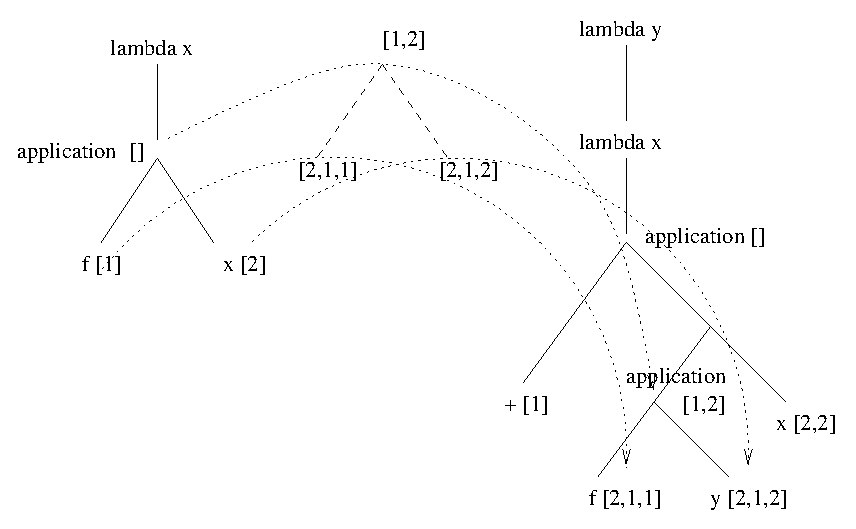
\epsfig{file=embed.eps, width=3in}
\end{center}
\caption{An Embedding}
\label{fig:embed}
\end{figure}

The embedding tree for this is  (node [1, 2] [(leaf
[1, 1, 1]) (leaf [2, 1, 2])])).  This states
that the function 
application at the top of $f(x)$ matches with the node at
address [1, 2] of $f(y) + x$ (i.e. the application involving $+$ has
been bypassed), that the
function symbol $f$ matches the sub term at [2,1,1] (i.e. $f$)
and $x$ matches $y$ (i.e.\ the bound variables can be consistently
renamed in either (or both) terms so that they are identical).

The annotations originally used in rippling 
are still useful for presentation.  Annotations consist of contexts
(expressions 
with holes) indicated by a wave front (box) with a directional arrow.
The holes in the context are wave holes (i.e. they are filled with an
expression which is underlined). The skeleton is everything
that appears outside wave fronts, or in wave holes. 
So the above embedding can be
presented as 
$$
\lam{x} \wfout{\lam{y} \wh{f(y)} + x}.
$$

NB.  It is important to remember that the annotations do not actually
exist in the implementation which records instead the 
skeleton and embedding\footnote{In fact \lclam\ maintains a list of
possible embeddings 
during rippling since there may be more than one way to embed the
induction hypotheses into the conclusion.  For convenience we assume
here there is only one.}.  
In some cases it is less easy to use the
traditional annotations to represent embeddings, particularly when dealing
with $\lambda$-abstrations which are ignored by the embedding trees.
You can see that in the above the bound variables in the skeleton 
are assumed to have been appropriately renamed already.
These 
annotations are just a presentational convenience.
\end{example}

\section{Logics}
You will note that the proof strategy for induction calls the {\tt
  taut}\index{taut} method for tautology checking.  This may vary
depending upon whether constructive or classical logic (for instance)
is being used.  As a result the basic ``build'' of the induction
theory\index{induction theory} in \lclam\ does not specify how the
{\tt taut} method or logical constants such as {\tt
  forall}\index{forall} or {\tt and}\index{and} should be treated by
the system.  It simply asserts that they exist.  Additional files, of
which the {\tt constructive\_logic}\index{constructive\_logic} theory
can then be created to provide the necessary details.

\section{Arithmetic, Natural Numbers and Lists}
There are a number of built-in theories dealing with natural number
and list theorems.  Standard functions and goals can be found in the
{\tt arithmetic}\index{arithmetic} theory and the {\tt
  objlists}\index{objlists} theory.  Further functions can be found in 
{\tt list\_benchmarks}\index{list\_benchmarks}, {\tt
  map\_benchmarks}\index{map\_benchmarks} and the {\tt
  clam\_corpus}\index{clam\_corpus} theories (there are 3 clam corpus
theory files).

\section{Mutual induction}
\noindent 
This module was written for the MFOTL group based at Liverpool.  The
method \texttt{alexei\_meth} in
\texttt{theories/mutual\_induction.mod} implements the following proof
rule.  It is a variant of a mutual induction rule suitable for
treatment of arithmetical translations of temporal formulae:

\vspace{0.5cm}

$ \forall y \forall \bar{x} A_{1}(y, \bar{x}) \Rightarrow B_{1}(s(y), \bar{x})$

$\forall y \forall \bar{x} A_{2}(y, \bar{x}) \Rightarrow B_{2}(s(y), \bar{x})$

$\ldots $

$\forall y \forall \bar{x} A_{n}(y, \bar{x}) \Rightarrow B_{n}(s(y), \bar{x})$

\vspace{-1mm}
$\underline{\qquad\qquad\qquad\qquad\qquad\qquad\qquad\qquad\qquad\qquad}$
 
\vspace{1mm}
$\forall u. u > t \Rightarrow \varphi(u)$ 

\vspace{5mm}
\noindent
with the side conditions: 

\[\begin{array}{l} 
\exists \bar{x}  (A_{1}(t,\bar{x}) \vee A_{2}(t, \bar{x}) \vee \ldots \vee 
A_{n}(t,\bar{x})) \\
\\
\forall y \forall \bar{x} (B_{i}(y, \bar{x}) \Rightarrow \varphi(y)) , i=1, \ldots, n \\
\\
\forall y \forall \bar{x} \exists \bar{z} ( B_{i}(y, \bar{x}) 
\Rightarrow \bigvee_{j=1\ldots n} A_{j}(y,\bar{z})) ,  i=1 \ldots, n 
\end{array}\]

\noindent
where $A_{i}$ and $B_{i}$ are arbitrary first-order formulae, $t$ is
an arbitrary arithmetical term, s is the successor function symbol,
$\Rightarrow$ is implication, $\bar{x}$ is a sequence of
variables, and $y$ is a (numerical) variable of type \texttt{nat}.  $n$ is
not fixed, so we can deal with arbitrary lists of premises in the rule.

\noindent
Since the rule is generally used in backward reasoning, 
one can present its application as follows: \\

\noindent
Given a goal sequent $H \vdash \psi$ with $\psi$ being of the form of
the conclusion of the above rule, the method generates some subset
$H'$ of $H$ matching the premises of the rule and generates the
associated side conditions as new subgoals.  These subgoals are
then resolved by application of some other methods (for first-order
reasoning). \\

\noindent
At present the method simply chooses the maximal matching subset of
hypotheses.  Probably some optimization for iteration over subsets
will be needed later.

\noindent{\bf Example:} \\

Given:   
\[\begin{array}{l}
\forall x, y (A(y,x) \Rightarrow B(s(y),x)) \\
\forall x, y (C(y,x) \Rightarrow D(s(y),x)) \\
\forall x (A(0,x) \lor C(0,x)) \\
\forall x,y (B(y,x) \Rightarrow C(y,x)) \\
\forall x,y (D(y,x) \Rightarrow (A(y,x) \lor C(y,x))) 
\end{array}\]

\vspace{-1mm}
$\underline{\qquad\qquad\qquad\qquad\qquad\qquad\qquad\qquad\qquad\qquad\qquad}$

Prove: 
\[\forall y > 0  \exists x (B(y,x) \lor D(y,x)) \]
 
Side conditions to prove (taking the set of first two hypotheses and the
conclusion):

\[\begin{array}{l}
\exists x (A(0,x) \lor C(0,x))\\
\\
\forall y \forall x (B(y,x) \Rightarrow  \exists z (B(y,z) \lor D(y,z))) \\
\\
\forall y \forall x (D(y,x) \Rightarrow  \exists z (B(y,z) \lor D(y,z))) \\
\\
\forall y \forall x \exists z (B(y,x) \Rightarrow A(y,z) \lor C(y,z)) \\
\\
\forall y \forall x \exists z (D(y,x) \Rightarrow A(y,z) \lor C(y,z)) \\
\end{array}\]